% Draft, 2 Nov 2026.  Build: pdflatex main.tex (twice).  Numbers: python3 ../floor/make_numbers.py regenerates
% numbers.tex, depth_table.tex and params_d*.tex from the saved optimiser points.
% Optional section (Nick to decide): set \includefloorfalse below.
\documentclass[11pt]{article}
\usepackage[margin=1in]{geometry}
\usepackage{amsmath,amssymb,amsthm,booktabs,hyperref,array,xcolor,graphicx,tikz}
\newtheorem{theorem}{Theorem}
\newtheorem{lemma}[theorem]{Lemma}
\newtheorem{proposition}[theorem]{Proposition}
\newtheorem{heuristic}{Heuristic}
\theoremstyle{definition}
\newtheorem{definition}[theorem]{Definition}
\theoremstyle{remark}
\newtheorem{remark}[theorem]{Remark}
\newcommand{\Z}{\mathbb{Z}}
\newcommand{\cD}{\mathcal{D}}
\newcommand{\Ot}{\widetilde{O}}
\hypersetup{hidelinks}
\newcommand{\todo}[1]{\textcolor{red}{[\textsc{todo}: #1]}}
\newif\ifincludefloor \includefloorfalse     % Section: list-size floor   -- Nick to decide
% generated by floor/make_numbers.py -- do not edit by hand
\newcommand{\THGJUone}{0.4056}
\newcommand{\THGJUtwo}{0.3371}
\newcommand{\THGJUthree}{0.3371}
\newcommand{\THGJUfour}{0.3371}
\newcommand{\THGJUfive}{0.3371}
\newcommand{\THGJUsix}{0.3371}
\newcommand{\THGJUseven}{0.3371}
\newcommand{\THGJUeight}{0.3371}
\newcommand{\THGJFone}{0.4056}
\newcommand{\THGJFtwo}{0.3269}
\newcommand{\THGJFthree}{0.3269}
\newcommand{\THGJFfour}{0.3269}
\newcommand{\THGJFfive}{0.3269}
\newcommand{\THGJFsix}{0.3269}
\newcommand{\THGJFseven}{0.3269}
\newcommand{\THGJFeight}{0.3269}
\newcommand{\TBCJUone}{0.4056}
\newcommand{\TBCJUtwo}{0.3122}
\newcommand{\TBCJUthree}{0.2891}
\newcommand{\TBCJUfour}{0.2891}
\newcommand{\TBCJUfive}{0.2891}
\newcommand{\TBCJUsix}{0.2891}
\newcommand{\TBCJUseven}{0.2891}
\newcommand{\TBCJUeight}{0.2891}
\newcommand{\TBCJFone}{0.4056}
\newcommand{\TBCJFtwo}{0.3122}
\newcommand{\TBCJFthree}{0.2852}
\newcommand{\TBCJFfour}{0.2814}
\newcommand{\TBCJFfive}{0.2814}
\newcommand{\TBCJFsix}{0.2814}
\newcommand{\TBCJFseven}{0.2814}
\newcommand{\TBCJFeight}{0.2814}
\newcommand{\TBBSSUone}{0.4056}
\newcommand{\TBBSSUtwo}{0.3025}
\newcommand{\TBBSSUthree}{0.2831}
\newcommand{\TBBSSUfour}{0.2831}
\newcommand{\TBBSSUfive}{0.2831}
\newcommand{\TBBSSUsix}{0.2831}
\newcommand{\TBBSSUseven}{0.2831}
\newcommand{\TBBSSUeight}{0.2831}
\newcommand{\TBBSSFone}{0.4056}
\newcommand{\TBBSSFtwo}{0.3025}
\newcommand{\TBBSSFthree}{0.2793}
\newcommand{\TBBSSFfour}{0.2744}
\newcommand{\TBBSSFfive}{0.2730}
\newcommand{\TBBSSFsix}{0.2722}
\newcommand{\TBBSSFseven}{0.2721}
\newcommand{\TBBSSFeight}{0.2721}
\newcommand{\TFiveUone}{\todo{run}}
\newcommand{\TFiveUtwo}{\todo{run}}
\newcommand{\TFiveUthree}{\todo{run}}
\newcommand{\TFiveUfour}{\todo{run}}
\newcommand{\TFiveUfive}{\todo{run}}
\newcommand{\TFiveUsix}{\todo{run}}
\newcommand{\TFiveUseven}{\todo{run}}
\newcommand{\TFiveUeight}{\todo{run}}
\newcommand{\TFiveFone}{\todo{run}}
\newcommand{\TFiveFtwo}{\todo{run}}
\newcommand{\TFiveFthree}{\todo{run}}
\newcommand{\TFiveFfour}{0.2739}
\newcommand{\TFiveFfive}{0.2727}
\newcommand{\TFiveFsix}{0.2721}
\newcommand{\TFiveFseven}{0.2721}
\newcommand{\TFiveFeight}{0.2721}
\newcommand{\TThreeUone}{\todo{run}}
\newcommand{\TThreeUtwo}{\todo{run}}
\newcommand{\TThreeUthree}{\todo{run}}
\newcommand{\TThreeUfour}{\todo{run}}
\newcommand{\TThreeUfive}{\todo{run}}
\newcommand{\TThreeUsix}{\todo{run}}
\newcommand{\TThreeUseven}{\todo{run}}
\newcommand{\TThreeUeight}{\todo{run}}
\newcommand{\TThreeFone}{\todo{run}}
\newcommand{\TThreeFtwo}{\todo{run}}
\newcommand{\TThreeFthree}{\todo{run}}
\newcommand{\TThreeFfour}{0.2742}
\newcommand{\TThreeFfive}{0.2732}
\newcommand{\TThreeFsix}{0.2732}
\newcommand{\TThreeFseven}{0.2732}
\newcommand{\TThreeFeight}{0.2732}
\newcommand{\TNineUone}{\todo{run}}
\newcommand{\TNineUtwo}{\todo{run}}
\newcommand{\TNineUthree}{\todo{run}}
\newcommand{\TNineUfour}{\todo{run}}
\newcommand{\TNineUfive}{\todo{run}}
\newcommand{\TNineUsix}{\todo{run}}
\newcommand{\TNineUseven}{\todo{run}}
\newcommand{\TNineUeight}{\todo{run}}
\newcommand{\TNineFone}{\todo{run}}
\newcommand{\TNineFtwo}{\todo{run}}
\newcommand{\TNineFthree}{\todo{run}}
\newcommand{\TNineFfour}{\todo{run}}
\newcommand{\TNineFfive}{\todo{run}}
\newcommand{\TNineFsix}{\todo{run}}
\newcommand{\TNineFseven}{\todo{run}}
\newcommand{\TNineFeight}{\todo{run}}
\newcommand{\TBBSSFthreeParked}{0.2793}
\newcommand{\TBBSSpublished}{0.2830}
\newcommand{\Tbest}{0.2721}
\newcommand{\Tbestdepth}{7}
\newcommand{\Twidebest}{0.2727}
\newcommand{\GainFilters}{0.0038}
\newcommand{\GainDepth}{0.0072}
\newcommand{\GainTotal}{0.0110}
\newcommand{\GainFiltersPct}{35}
\newcommand{\GainDepthPct}{65}
\newcommand{\Srcfour}{floor/runs/polish/gen\_m4\_4\_f\_11.npy}
\newcommand{\RootExcessfour}{0.119}
\newcommand{\Sonefour}{-0.059}
\newcommand{\Srcfive}{floor/runs/polish/gen\_m4\_5\_f\_11.npy}
\newcommand{\RootExcessfive}{0.118}
\newcommand{\Sonefive}{-0.059}
\newcommand{\Srcsix}{floor/runs/polish/gen\_m4\_6\_f\_51.npy}
\newcommand{\RootExcesssix}{0.104}
\newcommand{\Sonesix}{-0.052}
\newcommand{\Srcseven}{floor/runs/polish/gen\_m4\_7\_f\_41.npy}
\newcommand{\RootExcessseven}{0.104}
\newcommand{\Soneseven}{-0.052}
\newcommand{\BiasOffSigma}{0.8638}
\newcommand{\BiasOffPlanted}{0.8633}
\newcommand{\BiasOnSigma}{0.7150}
\newcommand{\BiasOnPlanted}{0.7200}
\newcommand{\BiasOnSE}{0.0259}
\newcommand{\SiboffTwentyFour}{-0.0056}
\newcommand{\SibindepTwentyFour}{+0.0039}
\newcommand{\SibsharedTwentyFour}{+0.0005}
\newcommand{\SiboffThirtyTwo}{+0.0009}
\newcommand{\SibindepThirtyTwo}{-0.0139}
\newcommand{\SibsharedThirtyTwo}{+0.0091}
\newcommand{\SiboffForty}{-0.0048}
\newcommand{\SibindepForty}{-0.0035}
\newcommand{\SibsharedForty}{-0.0048}
\newcommand{\SiboffFortyEight}{-0.0023}
\newcommand{\SibindepFortyEight}{-0.0005}
\newcommand{\SibsharedFortyEight}{+0.0077}


\title{Filtered merges make deeper representation trees pay:\\ random Subset Sum in \texorpdfstring{$2^{\Tbest n}$}{2\^{}(\Tbest n)}}
\author{Nick Howgrave-Graham}
\date{November 2026}
\setlength{\emergencystretch}{2em}
\begin{document}
\maketitle

\begin{abstract}
For random Subset Sum at density one, the best published heuristic exponent is $0.2830$, due to Bonnetain, Bricout,
Schrottenloher and Shen (BBSS), using representations with digit set $\{-1,0,1,2\}$. We add type-class
(consistency) filters, in the line of Dubiner and of May and Ozerov, to the merges of the BBSS tree. At the BBSS depth
the gain is small ($0.2830\to\TBBSSFthree$). However, the filters remove the reason why deeper trees did not help: in
the unfiltered tree the upper merges stay the most expensive whatever the depth, whereas filtered upper merges are
cheap enough for extra levels to pay. Depth $4$ already gives $\TBBSSFfour$; the best point we computed is $\Tbest$, at depth
$\Tbestdepth$, and the exponent converges to about $0.272$ as the depth grows, under the standard heuristics. We check the accounting against a survival recursion that every
reported optimum satisfies, prove that the filters cannot bias the survival of the planted solution, and test the
remaining independence assumptions by simulation. The filters pay exactly at the merges where most matched pairs
have the wrong split pattern.
\end{abstract}

\section{Introduction}
An instance of Subset Sum consists of integers $a_1,\dots,a_n$ and a target $t$, and asks for $x\in\{0,1\}^n$ with
$\langle a,x\rangle=t$. In the \emph{random} setting the $a_i$ are uniform in $[0,2^n)$ and $t=\langle a,x_0\rangle$
for a planted $x_0$ of weight $n/2$ (density one). We measure the exponent $\log_2(\text{time})/n$.

Meet-in-the-middle~\cite{HS74,SS81} gives $2^{n/2}$. Howgrave-Graham and Joux~\cite{HGJ10} introduced
\emph{representations}: the solution is written in many ways as a sum of two vectors, so a random modular constraint
can be imposed on the summands while some representation survives. Becker, Coron and Joux~\cite{BCJ11} allowed
digits $-1$, and Bonnetain, Bricout, Schrottenloher and Shen~\cite{BBSS20} added the digit $2$ and an accounting in
which intermediate lists may be random subsets of their constrained sets. Table~\ref{tab:history} summarises.

\begin{table}[ht]
\centering
\begin{tabular}{lllll}
\toprule
exponent & work & digit set & depth & merges \\
\midrule
$0.337$ & HGJ~\cite{HGJ10} (as corrected in~\cite{BCJ11}) & $\{0,1\}$ & 3 & plain \\
$0.329$ & May--Ozerov~\cite{Oze16} & $\{0,1\}$ & 2 & consistency filtered \\
$0.291$ & BCJ~\cite{BCJ11} & $\{-1,0,1\}$ & 3 & plain \\
$0.287$ & May--Ozerov~\cite{Oze16} & $\{-1,0,1\}$ & 3 & consistency filtered \\
$\TBCJFthree$, $\TBCJFfour$ & this work$^\dagger$ & $\{-1,0,1\}$ & 3, 4 & type-class filtered \\
\addlinespace
$0.2830$ & BBSS~\cite{BBSS20} & $\{-1,0,1,2\}$ & 3 & plain \\
\midrule
$\TBBSSFthree$ & this work & $\{-1,0,1,2\}$ & 3 & type-class filtered \\
$\TBBSSFfour$ & this work & $\{-1,0,1,2\}$ & 4 & type-class filtered \\
$\Tbest$ & this work & $\{-1,0,1,2\}$ & $\Tbestdepth$ & type-class filtered \\
\bottomrule
\end{tabular}
\caption{Heuristic time exponents for random density-one Subset Sum. Depth is the number of levels of
representation lists below the root ($d$ in Section~\ref{sec:prelim}); BBSS's ``five levels, numbered 4 down to
0''~\cite[\S2.5]{BBSS20} is $d=3$ with meet-in-the-middle leaves; our recomputation of~\cite{BBSS20} gives $0.2831$
(Table~\ref{tab:depth}). $^\dagger$BBSS accounting (Heuristic~\ref{heur:lists}); under the strict
accounting of~\cite{BCJ11}, which~\cite{Oze16} also uses, our filtered depth-3 value is $0.2864$, and
Ozerov's accounting gives HGJ $0.340$ rather than $0.337$, so the rows are not directly comparable.}
\label{tab:history}
\end{table}

\paragraph{The story.} At each merge of a representation tree, two lists are joined on a modular constraint, and
only a small fraction of the matching pairs have the right coordinate pattern. Filtering the pairs by their joint
coordinate type, so that inconsistent pairs are never generated, is the consistency technique of May and
Ozerov~\cite{Oze16}, which goes back to Dubiner's bucketing codes~\cite{Dub10}. On the BBSS tree at its own depth it
gains only about $0.004$. BBSS observed~\cite[Remark~4]{BBSS20} that the time ``is a decreasing function of the number
of levels, which quickly reaches a minimum'', because ``adding one more level does not change the cost of the upper
levels, which will remain the most expensive''; Ozerov makes the same observation for ternary trees~\cite[\S4.1]{Oze16}.
Filters change exactly this. They make the upper merges cheap, so additional levels, which shrink the lists, start to
pay, and at the optimum the costs of all merges tie. This gives the improvement
$0.2830\to\Tbest$ (Section~\ref{sec:results}): about $\GainFiltersPct\%$ of it comes from the filters at fixed depth,
and $\GainDepthPct\%$ from the depth they make affordable. In decoding the analogous effect is known: with
near-neighbour search at every level, BJMM-type trees improve up to depth~$4$~\cite{BM17b,BM18}.

\paragraph{What is new.} Filtering of representation trees is due to May and Ozerov~\cite{Oze16}, for the HGJ and BCJ
digit sets at depth at most $3$. Filters combined with depth are known in decoding, from Both and May~\cite{BM17b,BM18}.
New here are filters on the BBSS digit set $\{-1,0,1,2\}$, trees of depth $d\ge4$, and the soundness analysis.

\paragraph{Contributions.}
\begin{enumerate}
\item Type-class filtered $\tau$-merges on representation trees with general digit sets, with cost terms in closed
form and the observation that the filter law only matters through its label type (Section~\ref{sec:filter}).
\item An optimisation of the BBSS tree with filters at every merge, for depths $d\le8$: $\TBBSSFfour$ at depth $4$
and $\Tbest$ at depth $\Tbestdepth$, with the exponent converging to about $0.272$ (Section~\ref{sec:results}).
\item Soundness of the accounting: a survival recursion that is satisfied with equality by every reported optimum,
and a symmetry lemma showing that the planted solution survives each filtered merge with exactly the average
probability (Section~\ref{sec:sound}).
\item Experiments testing survival, filter bias and sibling independence (Section~\ref{sec:exp}).
\end{enumerate}
\paragraph{What is proved.} All results are heuristic, in the same sense as~\cite{HGJ10,BCJ11,BBSS20}. Proved are
Lemma~\ref{lem:filter}, Proposition~\ref{prop:cost} (given the heuristics), Remark~\ref{rem:piQ},
Proposition~\ref{prop:decode}, the survival recursion together with the check that every reported optimum satisfies
it, and Lemma~\ref{lem:sym}. Assumed are Heuristics~\ref{heur:lists} and~\ref{heur:filter}, which the experiments of
Section~\ref{sec:exp} support. Numerical are the exponents: each is the best point the optimiser found, not a proven
optimum of the model, and the depth limit of about $0.272$ is a fit.

\paragraph{Related work.} Consistency filtering for HGJ and BCJ trees is in Ozerov's thesis~\cite[Ch.~2,
\S4.2]{Oze16}, reporting joint work with May, which leaves digits $\pm2$ as an open question~\cite[after
Cor.~65]{Oze16}; BBSS list it as ``not studied''~\cite[Table~1]{BBSS20}. Böhme~\cite{Boh11} reportedly reached $0.2871$
with $\{-2,\dots,2\}$ (unpublished; see~\cite[fn.~5]{BBSS20}). Filtering by joint type is also the mechanism of
May--Ozerov near-neighbour search in decoding~\cite{MO15} and of the locality-sensitive filters of Becker, Ducas, Gama
and Laarhoven~\cite{BDGL16}; Christiani~\cite{Chr17} gives the asymmetric framework. In the decoding trees of Both and
May~\cite{BM17b,BM18} and the ternary-LWE trees of Kirshanova and May~\cite{KM21} (see~\cite[App.~A]{HKLS26} for a correction to its
analysis), near-neighbour search replaces exact
matching of values by approximate matching, and the representation coordinates are checked after each merge; our
filters act on the representation coordinates and keep exact modular matching. An earlier claim of
$2^{0.255n}$~\cite{EM19} has been withdrawn (``issue with counting duplicate representations''); unlike~\cite{EM19} we
never sample or modify list contents, and all representation counts are those of~\cite{BBSS20}.
Li~\cite{Li25} claims $2^{0.24n}$ using a ternary-tree representation structure; we were not able to reproduce this
exponent within the heuristics used here.

\section{Preliminaries}\label{sec:prelim}
Logarithms are to base $2$ and $H$ is Shannon entropy. For a finite set $\Sigma$ and $v\in\Sigma^n$ the \emph{type} of
$v$ is its empirical distribution; there are $2^{nH(P)+O(\log n)}$ strings of type $P$~\cite{CK11}. Exponents are
stated up to $O(\log n)/n$.

\paragraph{Digit sets, sets and merges.} A \emph{digit set} is a finite $\cD\subset\Z$ containing $0$ and $1$; we use
$\{-1,0,1,2\}$ unless stated otherwise. For a modulus $m$, residue $\tau\in\Z_m$ and type $w$ on $\cD$, the
\emph{$(m,\tau,w)$-set} is $\{x\in\cD^n:\ \mathrm{type}(x)=w,\ \langle a,x\rangle\equiv\tau\pmod m\}$.
A \emph{$\tau$-merge} of lists $L_A\subseteq$ an $(m',\tau_A,w')$-set and $L_B\subseteq$ an $(m',\tau-\tau_A,w')$-set, with
$m'\mid m$, outputs the $x+y$ ($x\in L_A$, $y\in L_B$) with $\langle a,x+y\rangle\equiv\tau\pmod m$ and
$\mathrm{type}(x+y)=w$, i.e.\ elements of the $(m,\tau,w)$-set. Outputs are kept as a set (no duplicates).

\paragraph{The tree of depth $d$.} Level $0$ is the solution $x_0$, of type $\delta_0=(\tfrac12,\tfrac12)$ on $\{0,1\}$.
Levels $j=1,\dots,d$ carry $2^j$ lists of type-$\delta_j$ vectors, constrained modulo $M_j=2^{c_jn}$ with
$1=c_0\ge c_1\ge\dots\ge c_d\ge0$, $M_j\mid M_{j-1}$, and residues chosen at random consistently down the tree (the
$\tau$'s). Each level-$(j-1)$ list is the $\tau$-merge of two level-$j$ lists; the level-$d$ lists are built by
meet-in-the-middle from half-vectors, in time $2^{H(\delta_d)n/2}$. The depth $d$ is the number of
levels of lists below the root.

\paragraph{Splits.} A level-$(j-1)$ digit $z$ is written $z=x+y$ with $x,y\in\cD$; the \emph{split law} $\sigma_j$ is
the joint type of $(x,y)$ over all coordinates. It is symmetric, has both marginals $\delta_j$, and is determined by
$\delta_{j-1}$ and, for each parent digit, a distribution over its unordered splits (for $\{-1,0,1,2\}$: three free
fractions, $0\to(\pm1,\mp1)$, $1\to(2,-1)$, $2\to(1,1)$). Write $H_j=H(\delta_j)$. A fixed level-$(j-1)$ vector has
$2^{\rho_jn}$ representations of split type $\sigma_j$, and a random pair of type-$\delta_j$ vectors is such a split
with probability $2^{p_jn}$, where
\[
\rho_j=H(\sigma_j)-H_{j-1},\qquad p_j=H(\sigma_j)-2H_j .
\]

\begin{heuristic}[BBSS~\cite{BBSS20}]\label{heur:lists}
Every list behaves like a uniformly random subset, of its stated size, of its $(M_j,\tau,\delta_j)$-set. The merge of
two level-$j$ lists of size $2^{\ell_jn}$ examines $2^{P_jn}$ pairs, $P_j=2\ell_j-(c_{j-1}-c_j)$, and outputs
$2^{(P_j+p_j)n}$ vectors; the expected number of solutions found at the root is at least $1$.
\end{heuristic}

\section{Filtered $\tau$-merges}\label{sec:filter}
Fix a merge of two level-$j$ lists and drop the index. Let $(X,Y)\sim\sigma$, and let $\Lambda$ take values in a
finite \emph{label set} with conditional law $\kappa(\cdot\mid x,y)$ (one law per ordered pair type). Write $Q$ for the
law of $(X,Y,\Lambda)$ and $Q_\Lambda$ for its label marginal.

\begin{definition}
A \emph{filter} is a string $u$ in the label set, of type $Q_\Lambda$. A left vector $x$ \emph{enters} $u$ if the joint
type of $(x,u)$ is the $(X,\Lambda)$-marginal of $Q$, and a right vector $y$ enters $u$ if the joint type of $(y,u)$
is the $(Y,\Lambda)$-marginal. The filtered $\tau$-merge draws $F=2^{I(XY;\Lambda)n}$ random filters and, within
each, matches the entering left and right vectors on the new constraint bits.
\end{definition}
These are Dubiner's random bucketing codes~\cite{Dub10}, specialised to a representation merge; with a two-symbol
label set and recursive block structure they are Ozerov's consistency algorithm~\cite[\S2.2]{Oze16}.
Figure~\ref{fig:merge} compares the two merges.

\begin{figure}[ht]
\centering
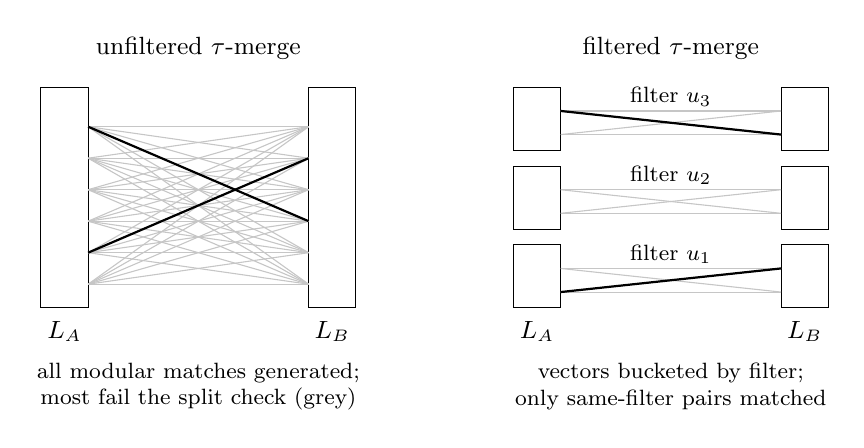
\begin{tikzpicture}[x=1cm,y=1cm,font=\small]
  \node at (2,3.3) {unfiltered $\tau$-merge};
  \draw (0,0) rectangle (0.6,2.8); \node at (0.3,-0.3) {$L_A$};
  \draw (3.4,0) rectangle (4,2.8); \node at (3.7,-0.3) {$L_B$};
  \foreach \i in {0.3,0.7,...,2.6} \foreach \k in {0.3,0.7,...,2.6}
    \draw[gray!45] (0.6,\i) -- (3.4,\k);
  \draw[thick] (0.6,0.7) -- (3.4,1.9); \draw[thick] (0.6,2.3) -- (3.4,1.1);
  \node[align=center,font=\footnotesize] at (2,-1.0) {all modular matches generated;\\ most fail the split check (grey)};
  \begin{scope}[xshift=6cm]
  \node at (2,3.3) {filtered $\tau$-merge};
  \foreach \b/\y in {1/0, 2/1, 3/2} {
    \draw (0,\y) rectangle (0.6,\y+0.8); \draw (3.4,\y) rectangle (4,\y+0.8);
    \node[font=\footnotesize] at (2,\y+0.68) {filter $u_\b$};
    \foreach \i in {0.2,0.5} \foreach \k in {0.2,0.5} \draw[gray!45] (0.6,\y+\i) -- (3.4,\y+\k);
  }
  \draw[thick] (0.6,0.2) -- (3.4,0.5); \draw[thick] (0.6,2.5) -- (3.4,2.2);
  \node at (0.3,-0.3) {$L_A$}; \node at (3.7,-0.3) {$L_B$};
  \node[align=center,font=\footnotesize] at (2,-1.0) {vectors bucketed by filter;\\ only same-filter pairs matched};
  \end{scope}
\end{tikzpicture}
\caption{Schematic of a $\tau$-merge without and with filters. Thick lines are valid splits, grey lines are matched
pairs with the wrong split pattern. With filters, each vector is placed in the filters it enters and only pairs that
share a filter are matched, so most of the wasted pairs are never generated.}
\label{fig:merge}
\end{figure}

\begin{lemma}\label{lem:filter}
Up to $2^{O(\log n)}$: a pair of joint type $\sigma$ enters a common random filter with probability
$2^{-I(XY;\Lambda)n}$; a left (right) vector enters with probability $2^{-I(X;\Lambda)n}$ ($2^{-I(Y;\Lambda)n}$); a
pair of independent type-$\delta$ vectors enters a common filter with probability $2^{-(I(X;\Lambda)+I(Y;\Lambda))n}$.
\end{lemma}
\begin{proof}
Method of types, as in~\cite{Dub10}: for fixed $(x,y)$ of type $\sigma$, $2^{nH(\Lambda\mid XY)}$ of the
$2^{nH(\Lambda)}$ strings of type $Q_\Lambda$ have joint type $Q$ with it; similarly for single vectors; for
independent $x,y$ the two events are independent given $u$.
\end{proof}

\begin{heuristic}\label{heur:filter}
The pairs that agree on the constraint bits behave, with respect to filters, like independent uniform pairs of
type-$\delta$ vectors.
\end{heuristic}

\begin{proposition}\label{prop:cost}
Under Heuristics~\ref{heur:lists} and~\ref{heur:filter}, the filtered $\tau$-merge outputs $2^{(P+p)n}$ vectors up to a
constant factor, at cost dominated by
\[
\underbrace{\ell+I(XY;\Lambda)-I(X;\Lambda)}_{\text{entries (left)}},\quad
\underbrace{\ell+I(XY;\Lambda)-I(Y;\Lambda)}_{\text{entries (right)}},\quad
\underbrace{P+I(XY;\Lambda)-I(X;\Lambda)-I(Y;\Lambda)}_{\text{pairs passing}},
\]
plus the cost of decoding, for each vector, the filters it enters.
\end{proposition}
With $F=2^{I(XY;\Lambda)n}$ filters a valid pair shares $\Theta(1)$ filters in expectation, so a constant
fraction of valid pairs could be missed; we use $nF$ filters, which makes the miss probability $e^{-\Omega(n)}$ per
pair at a polynomial cost. A filter pays when $I(X;\Lambda)+I(Y;\Lambda)>I(XY;\Lambda)$; we call $I(X;\Lambda)+I(Y;\Lambda)-I(XY;\Lambda)$ the
\emph{saving} of the merge.

\begin{remark}[Only the label type matters]\label{rem:piQ}
One may draw filters i.i.d.\ from any law $\pi$ on the label set; the number of filters and the entry probabilities
then change by factors $2^{\pm D(Q_\Lambda\|\pi)n}$ that cancel in all three cost terms, since only filters of type
$Q_\Lambda$ ever contain a valid pair. We therefore normalise $\pi=Q_\Lambda$ (see also Appendix~\ref{app:repro}).
\end{remark}

\paragraph{Decoding the filters.} Each vector must find the $2^{(I(XY;\Lambda)-I(X;\Lambda))n}$ filters it enters,
among $2^{I(XY;\Lambda)n}$, in time close to that number. Random codes do not allow this, so we use a product
construction, as in Dubiner's bucketing codes~\cite{Dub10} and the tensored filters of~\cite{BDGL16}; it does not
need the code rates to be small.

\begin{proposition}\label{prop:decode}
The filtered $\tau$-merge can be implemented so that each cost term of Proposition~\ref{prop:cost} is achieved up to
a factor $2^{o(n)}$, including the time to decode the filters, while each valid pair of type $\sigma$ is still found
with probability $1-o(1)$.
\end{proposition}
\begin{proof}
Apply a uniformly random permutation to the coordinates (the instance is exchangeable) and cut them into
$b=\lceil\sqrt n\rceil$ blocks of size $s\ge\lfloor n/b\rfloor$. For a valid pair, the vector of its per-block joint
types, its \emph{pattern}, is a sequence $(\sigma_1,\dots,\sigma_b)$ averaging to $\sigma$. Call the pattern
\emph{typical} if $\|\sigma_i-\sigma\|_\infty\le\epsilon_n=n^{-1/4}\log n$ for every $i$. Fix a valid pair. After the
permutation, each block is a sample of $s$ coordinates drawn without replacement from its $n$ coordinates, so for each
joint digit type $t$ of the pair, Hoeffding's inequality for sampling without replacement~\cite[\S6]{Hoe63} gives
\[
\Pr\bigl[|\sigma_i(t)-\sigma(t)|>\epsilon_n\bigr]\le2e^{-2s\epsilon_n^2}=2e^{-2(1-o(1))\log^2n}=n^{-\Theta(\log n)} .
\]
A union bound over the $b$ blocks and the $O(1)$ joint types shows that the pattern is typical with probability
$1-O(\sqrt n)\,n^{-\Theta(\log n)}=1-o(1)$. The block types of $x$ and of $y$ are marginals of the pair's block
types, so they are within $\epsilon_n$ of $\delta$ as well. A block type takes at most $(s+1)^{O(1)}$ values, so there
are at most $(\sqrt n+1)^{O(b)}=2^{O(\sqrt n\log n)}$ typical patterns.

For each pattern we build an independent filter family: in block $i$, a random code $C_i$ of
$2^{\sqrt n\, I_{\sigma_i}(XY;\Lambda)}$ label strings of type $Q_{\Lambda,i}$ (the label marginal of
$\sigma_i\times\kappa$), and a filter is a tuple $(u_1,\dots,u_b)\in C_1\times\dots\times C_b$. A left vector enters the
tuple if it enters every $u_i$ in the sense of Section~\ref{sec:filter}, with block-$i$ marginals; similarly on the
right. A vector can only enter a tuple whose block marginals equal its own block types, so it enters only the
family of its own pattern, and a vector with an atypical pattern enters no family at all: atypical vectors add
nothing to the entry cost. Concentration is therefore needed only for valid pairs, and by the bound above a valid
pair is lost in this way with probability $o(1)$. A vector decodes its filters by testing, in each block, all of $C_i$ (time $2^{O(\sqrt n)}$) and then
enumerating the product of the per-block lists, in time proportional to the output plus $b\,2^{O(\sqrt n)}$.

Lemma~\ref{lem:filter} applies in each block. The probabilities multiply, so a valid pair with this pattern shares
$\Theta(1)$ filters in expectation (amplified as above), and the entry and passing exponents are block averages of the
single-block terms. Those terms are continuous functions of the pair type for fixed $\kappa$, so each average differs
from the global term of Proposition~\ref{prop:cost} by $O(\epsilon_n)$, i.e.\ by $o(n)$ in the exponent. Summing over
the $2^{o(n)}$ patterns multiplies all costs by $2^{o(n)}$.
\end{proof}

\section{Accounting and soundness}\label{sec:sound}
\paragraph{The program.} For fixed split laws and filter laws, the exponents $(c_j,\ell_j,T)$ are the variables of a
linear program: minimise $T$ subject to Heuristic~\ref{heur:lists} ($\ell_{j-1}=P_j+p_j$, $\ell_j+c_j\le H_j$, root
yield $\ge1$), nesting $c_j\le c_{j-1}$, and $T$ at least the leaf build $H_d/2$, every list size, and, at every merge,
the three terms of Proposition~\ref{prop:cost} (or $P_j$ if unfiltered). The split and filter laws are optimised by
repeated Powell and Nelder--Mead searches, warm-started from shallower optima, from deeper ones, and from optima
for wider digit sets with the extra digits projected out; each reported value is the best over all these starts.
The depth is fixed, with per-level constants; trees whose depth grows with $n$ are outside the model.

\paragraph{Survival recursion.} Heuristic~\ref{heur:lists} allows $c_j>\rho_j$ at a level (fewer representations
than the constraint removes), which is not obviously sound: a level-$(j-1)$ element then survives only with
probability $2^{-(c_j-\rho_j)n}$. Let $s_j\le0$ be the log-survival exponent of a level-$j$ element, with $s_d=0$
(complete leaves). Saturating the Poisson survival law $\sigma=1-e^{-c\sigma_A\sigma_B}$ gives
\[
s_j=\min\bigl(0,\ \rho_{j+1}-c_{j+1}+2s_{j+1}\bigr)\quad(j=d-1,\dots,1),\qquad
\rho_1-c_1+2s_1\ge0\ \text{(root)},
\]
with list sizes $\ell_j=H_j-c_j+s_j$. Excess representations at a split compensate deficits deeper in the tree
(closer to the leaves); since survival is capped at $1$, they cannot be carried upward to pay for a deficit closer to
the root. So the accounting of Heuristic~\ref{heur:lists} is sound exactly when every deficit lies below a
sufficient excess. We solve the program with these constraints in place of
Heuristic~\ref{heur:lists} (exactly, by enumerating which levels saturate). \textbf{Every reported optimum gives the same
value under both accountings.} At depth~$4$, only the split into level~$2$ has a deficit ($s_1=\Sonefour$), paid exactly by the root
excess $\rho_1-c_1=\RootExcessfour=-2s_1$ (Table~\ref{tab:params4}).

\paragraph{Symmetry.} Filtered lists are not uniform random subsets in any obvious sense, but the planted solution is
not disadvantaged.

\begin{lemma}\label{lem:sym}
Fix a node (per node), its exact type, and the randomness: the instance $a$ with i.i.d.\ uniform coordinates, the
node's residue $\tau$, marginally uniform and independent of $a$, the residues below it (functions of $\tau$ and fresh
independent randomness), and i.i.d.\ filters independent of all of these. Let $O$ be the output list and $V_\tau$ the parents
of the exact type in the node's residue class. Then for every parent $P$ of that type,
\[
\Pr[P\in O\mid P\in V_\tau]=\mathbb{E}|O|\,/\,\mathbb{E}|V_\tau| ,
\]
and the same holds at every level.
\end{lemma}
\begin{proof}
Every step (complete coset leaves, modular joins, validity checks, the exact-type output restriction, and filter
entry, which depends only on joint (digit, label) counts) is equivariant under coordinate permutations $g$:
$O(g a,\tau,g u)=g\,O(a,\tau,u)$. The law of $(a,\tau,u)$ is $g$-invariant and $g$ maps $V_\tau$ to itself, so
$\Pr[P\in O\wedge P\in V_\tau]$ is the same for all $P$ of the type, on which the permutations act transitively.
Summing over $P$ and dividing by $\Pr[P\in V_\tau]=1/M$ gives the claim; child lists are outputs of equivariant steps,
so induction over levels applies.

The hypothesis on residues holds in the planted model. The root target $t=\langle a,x_0\rangle$ depends on $a$, but at
every node the residue is $\tau$ or $t-\tau$ (reduced modulo the node's modulus) for a $\tau$ that is uniform and
independent of $(a,x_0)$, so each node residue is marginally uniform and independent of $a$. The planted parent $P^*$
at a node is a function of $x_0$ and of the split choices, so it is independent of $a$, and the lemma applies to it.
\end{proof}
The lemma concerns the ratio of expectations, which is the quantity the accounting uses; it says nothing about joint
survival of two nodes. In particular sibling residues $\tau$ and $t-\tau$ are dependent through $t$; this joint
dependence is what the sibling-independence experiment of Section~\ref{sec:exp} tests.

\section{Results}\label{sec:results}
\begin{table}[ht]
\centering
% generated by floor/make_numbers.py
\begin{tabular}{llcccccc}
\toprule
digit set & merges & $d=1$ & $2$ & $3$ & $4$ & $5$ & $6$ \\
\midrule
$\{0,1\}$ & plain & 0.4056 & 0.3371 & 0.3371 & 0.3371 & 0.3371 & 0.3371 \\
 & filtered & 0.4056 & 0.3269 & 0.3269 & 0.3269 & 0.3269 & 0.3269 \\
\midrule
$\{-1,0,1\}$ & plain & 0.4056 & 0.3122 & 0.2891 & 0.2891 & 0.2891 & 0.2891 \\
 & filtered & 0.4056 & 0.3122 & 0.2852 & 0.2814 & 0.2814 & 0.2814 \\
\midrule
$\{-1,0,1,2\}$ & plain & 0.4056 & 0.3025 & 0.2831 & 0.2831 & 0.2831 & 0.2831 \\
 & filtered & 0.4056 & 0.3025 & 0.2793 & 0.2744 & 0.2730 & 0.2726 \\
\bottomrule
\end{tabular}

\caption{Time exponents by depth $d$, BBSS accounting, plain and filtered merges (each entry is the best found; a
deeper tree can copy a shallower one, so entries are monotone). $\{0,1\}$ and $\{-1,0,1\}$ under BBSS accounting give
$0.3371$ and $0.2891$; the strict accounting of~\cite{HGJ10,BCJ11} gives $0.3371$ and $0.2909$.}
\label{tab:depth}
\end{table}

\begin{theorem}[heuristic]\label{thm:main}
Under Heuristics~\ref{heur:lists} and~\ref{heur:filter}, random density-one Subset Sum can be solved in time
$2^{(\Tbest+o(1))n}$ with a filtered $\{-1,0,1,2\}$ tree of depth $\Tbestdepth$, and in time
$2^{(\TBBSSFfour+o(1))n}$ with depth $4$. The $o(1)$ comes from filter decoding (Proposition~\ref{prop:decode}).
\end{theorem}

\paragraph{Structure of the optimum.} Table~\ref{tab:params4} gives the depth-4 point. The filtered passing costs of
all four merges tie at $T$. At this point the filters save $0.066$ and $0.049$ at the dense levels $1$--$2$, only $0.009$ at
level~$3$, and nothing at the last merge. The deficit at level $2$ is paid by the root excess, and the survival
recursion is tight. The deeper optima (Tables~\ref{tab:params5}--\ref{tab:params8}) filter at the dense top levels \emph{and} at the sparse level near the
bottom where $1\to(2,-1)$ splits dominate ($I(XY;\Lambda)=0.21$, $0.27$, $0.28$ at $d=5,6,7$). There the lists are
mostly zeros: at $d=6$ the bottom level has $\delta_6(1)=0.0049$ against $\delta_6(2)=0.0112$ and
$\delta_6(-1)=0.0194$, so it consists mainly of $2$s and $-1$s split from the level-$5$ ones. Lemma~\ref{lem:sym} holds at every level, sparse ones included,
so these merges need no separate bias argument (see also Section~\ref{sec:exp}).

\paragraph{Where filters pay.} The column $p_j=H(\sigma_j)-2H_j$ of the parameter tables is the log-probability that a
random matched pair is a valid split, and a filter can only save what this pattern waste costs. At the depth-$7$
point $p_j$ is $-0.33$ and $-0.09$ at the two top merges, $-0.05$ and $-0.005$ in the middle, and $-0.18$ at the sparse
level~$6$, and the savings follow the same profile. At the dense top levels a random pair has overlapping supports. At
the sparse bottom levels the dominant split $1\to(2,-1)$ needs a $2$ and a $-1$ on the same coordinate, which random
pairs rarely have. In the middle levels supports are sparse and the splits are mostly $1\to(1,0)$, so a random matched
pair is almost always valid and there is nothing to filter.

\paragraph{Memory.} The memory exponent, the largest of the leaf lists, the stored lists and the filter entries
$\ell_j+I(XY;\Lambda)-\min(I(X;\Lambda),I(Y;\Lambda))$, is $\Memfour$ at depth~$4$ and $\Memseven$ at depth~$7$
(last line of each parameter table). At every reported point it equals or nearly equals the time, because the entry
terms tie with the passing terms at the optimum. The gain over BBSS,
$\GainTotal$ (from our recomputed $0.2831$), splits into $\GainFilters$ from filters at depth $3$ and $\GainDepth$ from the extra depth.

\begin{table}[ht]
\centering\small
% generated by floor/make_numbers.py from floor/runs/polish/gen_m4_4_f_cloud.npy
\begin{tabular}{rcccccccc}
\toprule
$j$ & $\delta_j(-1)$ & $\delta_j(0)$ & $\delta_j(1)$ & $\delta_j(2)$ & $\rho_j$ & $c_j$ & $s_j$ & $\ell_j$ \\
\midrule
1 & 0.0534 & 0.6497 & 0.2905 & 0.0064 & 1.0285 & 0.8872 & -0.0707 & 0.2369 \\
2 & 0.0573 & 0.7614 & 0.1803 & 0.0010 & 0.7088 & 0.7794 & 0.0000 & 0.2124 \\
3 & 0.0523 & 0.8335 & 0.1136 & 0.0006 & 0.5449 & 0.5449 & 0.0000 & 0.2593 \\
4 & 0.0324 & 0.9040 & 0.0636 & 0.0000 & 0.2722 & 0.2722 & 0.0000 & 0.2727 \\
\bottomrule
\end{tabular}

\medskip

\begin{tabular}{rcccccc}
\toprule
merge of level $j$ & pairs & $p_j$ & $I(XY;\Lambda)$ & entries gap & saving & passing \\
\midrule
1 & 0.3611 & -0.3611 & 0.1601 & 0.0357 & -0.0886 & 0.2725 \\
2 & 0.3171 & -0.0801 & 0.1650 & 0.0603 & -0.0443 & 0.2727 \\
3 & 0.2841 & -0.0717 & 0.0382 & 0.0134 & -0.0114 & 0.2727 \\
4 & 0.2727 & -0.0134 & 0.0000 & 0.0000 & 0.0000 & 0.2727 \\
\bottomrule
\end{tabular}

\smallskip
{\footnotesize leaves $H_4/2 = 0.2725$;\quad root excess $\rho_1-c_1 = +0.1413$, $2s_1 = -0.1413$;\quad memory $0.2727$;\quad $T = 0.27272$}

\caption{The depth-4 optimum: levels (top) and merges (bottom). Columns:
$\delta_j(\cdot)$, the digit type of level $j$;
$\rho_j$, the representation exponent of a level-$(j-1)$ vector into level-$j$ pairs;
$c_j$, the constraint bits ($M_j=2^{c_jn}$);
$s_j$, the survival exponent of Section~\ref{sec:sound};
$\ell_j$, the list size;
\emph{pairs}, $P_j=2\ell_j-(c_{j-1}-c_j)$, the pairs an unfiltered merge would examine;
$p_j=H(\sigma_j)-2H_j$, the log-probability that a matched pair is a valid split;
$I(XY;\Lambda)$, the code rate (at $\pi=Q_\Lambda$);
\emph{entries gap}, $I(XY;\Lambda)-\min(I(X;\Lambda),I(Y;\Lambda))$, the log number of filters per vector;
\emph{saving}, $I(XY;\Lambda)-I(X;\Lambda)-I(Y;\Lambda)$ (negative means fewer pairs);
\emph{passing}, pairs $+$ saving, the pairs the filtered merge examines.
The last line gives the leaf build, the root condition and the memory exponent.
All exponents are per $n$.}
\label{tab:params4}
\end{table}

\paragraph{Saturation.} The exponent saturates with depth: $\TBBSSFthree$, $\TBBSSFfour$, $\TBBSSFfive$,
$\TBBSSFsix$, $\TBBSSFseven$, $\TBBSSFeight$ for $d=3,\dots,8$ (Table~\ref{tab:depth}). Each is a computed point, the
best found over all starts, not a proven optimum of the model, so $\Tbest$ is not a lower bound for it. The gains
shrink roughly geometrically. Fits of $T_d=T_\infty+Ar^d$ to subsets of these values give $T_\infty$ between $0.2719$
and $0.2724$ and $r$ between $0.14$ and $0.52$; the fit is sensitive to the last digits, which depend on the starting
point of the search, so we only claim that the exponent converges to about $0.272$. Deeper trees alone therefore do not lead to subexponential time within this accounting.

\paragraph{Wider digit sets.} Adding the digit $-2$ gains at most $0.0004$ at fixed depth ($0.2744\to0.2740$ at
$d=4$, $0.2730\to0.2727$ at $d=5$, and $0.0001$ at $d=6$ against a $\{-1,0,1,2\}$ re-optimisation from the same start);
the optimiser keeps a small positive $-2$ mass. The digit $3$ has zero marginal value, since it can only arise from
splitting a $2$, and an optimisation over $\{-4,\dots,4\}$ did not converge and was stopped. We therefore keep the BBSS
digit set $\{-1,0,1,2\}$ throughout.

\paragraph{Label sets.} Re-optimising the filters at depth $5$ with a $4$-symbol label set, warm-started from the
$3$-symbol optimum, gives $0.273224$ against $0.273335$: a gain of $0.0001$, so $3$-symbol filters appear essentially
optimal.

\section{Experimental validation}\label{sec:exp}
\paragraph{Survival.} Table~\ref{tab:survival}: a depth-3 HGJ tree (weights $n/2\to n/4\to n/8\to n/16$) with complete
leaves (leaf ratio $c\approx3.9$) and internal ratio $c\in\{1,2,3,4\}$. The Poisson model
$\sigma=1-e^{-c\sigma_A\sigma_B}$ is slightly optimistic at every level, but survival at $c=3$ does not decay, and the
work per success is flat in $c$ to within about one bit (conservation: raising $c$ buys nothing).
\begin{table}[ht]
\centering\small
\begin{tabular}{cccccccc}
\toprule
$n$ (draws) & $c$ & $\sigma_2$ & Poisson & $\sigma_1$ & Poisson & $\Pr[x_0\text{ found}]$ (Poisson) & $\log_2$ work/success \\
\midrule
48 (40) & 1 & 0.953 & 0.982 & 0.593 & 0.618 & 0.15 (0.32) & 21.3 \\
 & 2 & 0.954 & 0.982 & 0.823 & 0.856 & 0.65 (0.77) & 20.5 \\
 & 3 & 0.943 & 0.982 & 0.906 & 0.943 & 0.98 (0.93) & 20.8 \\
 & 4 & 0.957 & 0.982 & 0.957 & 0.979 & 1.00 (0.98) & 21.4 \\
\midrule
64 (10) & 1 & 0.963 & 0.980 & 0.602 & 0.617 & 0.30 (0.32) & 25.3 \\
 & 2 & 0.967 & 0.980 & 0.841 & 0.853 & 0.50 (0.77) & 26.0 \\
 & 3 & 0.953 & 0.980 & 0.928 & 0.944 & 0.90 (0.93) & 26.1 \\
 & 4 & 0.964 & 0.980 & 0.972 & 0.978 & 1.00 (0.98) & 26.6 \\
\bottomrule
\end{tabular}
\caption{Survival by level in a real HGJ tree (\texttt{floor/survival.py}). $\sigma_j=|L_j|/\mathbb{E}|V_j|$. At $n=64$
the modulus is capped at $2^{56}$ (density $1.14$).}
\label{tab:survival}
\end{table}

\paragraph{Filter bias.} A filtered merge at $n=32$ shaped like the level-2 merge of the optimum (complete coset
lists of about $1900$ elements, a $3$-symbol label set from the optimum's conditionals, $300$ draws): the planted
parent survives with probability $\BiasOffPlanted$ against mean $\sigma=\BiasOffSigma$ without filters, and
$\BiasOnPlanted\pm\BiasOnSE$ against $\BiasOnSigma$ with filters, as Lemma~\ref{lem:sym} predicts. A second merge at $n=20$ is shaped like
the sparse bottom merge of the depth-6 optimum: the parent has four $1$s and two $-1$s, and the children have two
$2$s and three $-1$s, joined by $1\to(2,-1)$ and $-1\to(-1,0)$ (\texttt{floor/bias\_sim\_sparse.py}, $400$ draws).
The planted parent survives with probability $0.598\pm0.025$ against $\sigma=0.611$ without filters, and
$0.438\pm0.025$ against $0.445$ with filters.

\paragraph{Sibling independence.} Two planted siblings (disjoint supports, shared instance, independent residues),
each built by its own filtered merge, $4000$ draws per $n$: $\Delta=\log_2\Pr[\text{both}]-\log_2\Pr[A]-\log_2\Pr[B]$
is $\SibsharedTwentyFour$, $\SibsharedThirtyTwo$, $\SibsharedForty$, $\SibsharedFortyEight$ at $n=24,32,40,48$ with
one shared code (similar with independent codes and without filters), all within $\pm0.02$ and with no trend in $n$.
So the exactly tight root condition needs no extra excess.

\ifincludefloor
\section{A list-size floor}\label{sec:floor}
% OPTIONAL (Nick to decide; \includefloortrue in main.tex).
\paragraph{(b) A list-size floor.} For trees with a two-way root and modular constraints only, a lower bound on any
cost is the largest list. At the first level, with the root split $S=A+B$ of law $P_{AB}$, the lists have size at least
$2^{(\max(H(A),H(B))-\min(1,H(A,B)-1))n}$, which minimises to $0.3113$, $0.1728$ and $0.1701$ for the digit sets
$\{0,1\}$, $\{-1,0,1\}$ and $\{-1,0,1,2\}$; type-class filters do not move it (data processing). With all levels and
the survival constraints but lists only, the floor rises to about $0.20$--$0.21$ for $d\le6$; adding the leaf build
gives $0.22$--$0.23$ at $d=6$. Adding merge costs gives the values of Table~\ref{tab:depth}. So the remaining gap from
about $0.21$ to $0.27$ is entirely merge cost, and a substantially better algorithm would need a structurally
different merge. \todo{numbers from floor/runs/rf\_*\_F0*.log; re-run the optimiser failures noted there}

\fi

\section{Conclusion and open problems}
Filters and depth attack the same waste from two sides, and together they give $\Tbest$; with depth the exponent
converges to about $0.272$. What remains is merge cost, so going substantially lower needs a structural change, such
as a non-binary root with a fast join, non-modular information, or a top level that is not enumerated, rather than
more depth. Open: quantum (walk or Grover) versions of filtered merges, as in~\cite{BBSS20}; non-binary roots and non-enumerative
top levels; wider digit sets, which add at most about $0.0004$ at fixed depth; and transferring the
observation to decoding and ternary-LWE trees, where merges also generate pairs with the wrong split pattern; for
Meet-LWE we found no gain at the published optima, where the binding merges have little split-pattern waste.
Lattice-based hybrids, such as guessing combined with batch-CVP, may be competitive at density one; whether they can be combined with filtered representation trees is open.

\appendix
\section{Parameters and reproduction}\label{app:repro}
In the numerical model the filter law $\pi$ is a free parameter; at one optimum it drifted to $\pi_N\approx0$, giving
formal code rates of $34n$ and $128n$ at two levels, while all costs were unchanged on resetting $\pi=Q_\Lambda$
(Remark~\ref{rem:piQ}). The rates in the tables are at $\pi=Q_\Lambda$.

Tables~\ref{tab:params5}--\ref{tab:params8} give the depth-5 to depth-8 points (columns as in
Table~\ref{tab:params4}). The points are stored as
\begin{center}\small\texttt{\Srcfour}\quad(depth 4)\\ \texttt{\Srcfive}\quad(depth 5)\\ \texttt{\Srcsix}\quad(depth 6)\\
\texttt{\Srcseven}\quad(depth 7)\\ \texttt{\Srceight}\quad(depth 8)\end{center}
All numbers in this paper are generated by
\texttt{floor/make\_numbers.py}; the model is \texttt{gen\_lsf.py}, the optimiser \texttt{gen\_opt.py}, and the
survival-recursion accounting \texttt{floor/recursive\_floor.py} (variants S1/S2).
\begin{table}[ht]
\centering\small
% generated by floor/make_numbers.py from floor/runs/polish/gen_m4_5_f_11.npy
\begin{tabular}{rcccccccc}
\toprule
$j$ & $\delta_j(-1)$ & $\delta_j(0)$ & $\delta_j(1)$ & $\delta_j(2)$ & $\rho_j$ & $c_j$ & $s_j$ & $\ell_j$ \\
\midrule
1 & 0.0445 & 0.6675 & 0.2814 & 0.0066 & 0.9708 & 0.8530 & -0.0589 & 0.2396 \\
2 & 0.0463 & 0.7844 & 0.1675 & 0.0019 & 0.6364 & 0.6953 & 0.0000 & 0.2335 \\
3 & 0.0387 & 0.8602 & 0.1008 & 0.0002 & 0.4362 & 0.4362 & 0.0000 & 0.2686 \\
4 & 0.0215 & 0.9257 & 0.0528 & 0.0000 & 0.1834 & 0.1702 & -0.0066 & 0.2697 \\
5 & 0.0247 & 0.9489 & 0.0125 & 0.0139 & 0.1270 & 0.1336 & 0.0000 & 0.2349 \\
\bottomrule
\end{tabular}

\medskip

\begin{tabular}{rcccccc}
\toprule
merge of level $j$ & pairs & $p_j$ & $I(XY;\Lambda)$ & entries gap & saving & passing \\
\midrule
1 & 0.3323 & -0.3323 & 0.1142 & 0.0269 & -0.0604 & 0.2718 \\
2 & 0.3093 & -0.0697 & 0.1153 & 0.0395 & -0.0362 & 0.2730 \\
3 & 0.2782 & -0.0447 & 0.0140 & 0.0044 & -0.0051 & 0.2730 \\
4 & 0.2734 & -0.0048 & 0.0070 & 0.0033 & -0.0004 & 0.2730 \\
5 & 0.4332 & -0.1635 & 0.2115 & 0.0244 & -0.1626 & 0.2706 \\
\bottomrule
\end{tabular}

\smallskip
{\footnotesize leaves $H_5/2 = 0.1842$;\quad root excess $\rho_1-c_1 = +0.1177$, $2s_1 = -0.1177$;\quad memory $0.2730$;\quad $T = 0.27305$}

\caption{The depth-5 point.}\label{tab:params5}
\end{table}
\begin{table}[ht]
\centering\small
% generated by floor/make_numbers.py from floor/runs/polish/gen_m4_6_f_51.npy
\begin{tabular}{rcccccccc}
\toprule
$j$ & $\delta_j(-1)$ & $\delta_j(0)$ & $\delta_j(1)$ & $\delta_j(2)$ & $\rho_j$ & $c_j$ & $s_j$ & $\ell_j$ \\
\midrule
1 & 0.0435 & 0.6689 & 0.2818 & 0.0059 & 0.9609 & 0.8568 & -0.0521 & 0.2343 \\
2 & 0.0487 & 0.7791 & 0.1707 & 0.0015 & 0.6619 & 0.7140 & 0.0000 & 0.2285 \\
3 & 0.0411 & 0.8555 & 0.1031 & 0.0003 & 0.4549 & 0.4549 & 0.0000 & 0.2680 \\
4 & 0.0227 & 0.9233 & 0.0539 & 0.0000 & 0.1885 & 0.1884 & -0.0001 & 0.2698 \\
5 & 0.0161 & 0.9568 & 0.0223 & 0.0047 & 0.1143 & 0.0666 & -0.0239 & 0.2255 \\
6 & 0.0194 & 0.9646 & 0.0049 & 0.0112 & 0.0427 & 0.0666 & 0.0000 & 0.2037 \\
\bottomrule
\end{tabular}

\medskip

\begin{tabular}{rccccc}
\toprule
merge of level $j$ & pairs & $I(XY;\Lambda)$ & entries gap & saving & passing \\
\midrule
1 & 0.3253 & 0.1221 & 0.0269 & -0.0682 & 0.2570 \\
2 & 0.3142 & 0.1294 & 0.0437 & -0.0420 & 0.2722 \\
3 & 0.2770 & 0.0131 & 0.0042 & -0.0047 & 0.2722 \\
4 & 0.2731 & 0.0058 & 0.0024 & -0.0009 & 0.2722 \\
5 & 0.3292 & 0.0872 & 0.0147 & -0.0579 & 0.2713 \\
6 & 0.4074 & 0.2737 & 0.0685 & -0.1367 & 0.2707 \\
\bottomrule
\end{tabular}

\smallskip
{\footnotesize leaves $H_6/2 = 0.1351$;\quad root excess $\rho_1-c_1 = +0.1042$, $2s_1 = -0.1042$;\quad $T = 0.27223$}

\caption{The depth-6 point.}\label{tab:params6}
\end{table}
\begin{table}[ht]
\centering\small
% generated by floor/make_numbers.py from floor/runs/polish/gen_m4_7_f_41.npy
\begin{tabular}{rcccccccc}
\toprule
$j$ & $\delta_j(-1)$ & $\delta_j(0)$ & $\delta_j(1)$ & $\delta_j(2)$ & $\rho_j$ & $c_j$ & $s_j$ & $\ell_j$ \\
\midrule
1 & 0.0438 & 0.6684 & 0.2819 & 0.0059 & 0.9631 & 0.8591 & -0.0520 & 0.2337 \\
2 & 0.0495 & 0.7786 & 0.1691 & 0.0027 & 0.6734 & 0.7254 & 0.0000 & 0.2272 \\
3 & 0.0423 & 0.8537 & 0.1033 & 0.0007 & 0.4654 & 0.4654 & 0.0000 & 0.2682 \\
4 & 0.0237 & 0.9214 & 0.0547 & 0.0001 & 0.1965 & 0.1965 & 0.0000 & 0.2711 \\
5 & 0.0144 & 0.9580 & 0.0251 & 0.0025 & 0.1050 & 0.0853 & -0.0099 & 0.2070 \\
6 & 0.0199 & 0.9649 & 0.0026 & 0.0126 & 0.0447 & 0.0545 & 0.0000 & 0.2099 \\
7 & 0.0118 & 0.9786 & 0.0035 & 0.0061 & 0.0545 & 0.0545 & 0.0000 & 0.1252 \\
\bottomrule
\end{tabular}

\medskip

\begin{tabular}{rccccc}
\toprule
merge of level $j$ & pairs & $I(XY;\Lambda)$ & entries gap & saving & passing \\
\midrule
1 & 0.3264 & 0.1458 & 0.0331 & -0.0796 & 0.2468 \\
2 & 0.3206 & 0.1384 & 0.0450 & -0.0485 & 0.2721 \\
3 & 0.2765 & 0.0121 & 0.0039 & -0.0044 & 0.2721 \\
4 & 0.2733 & 0.0032 & 0.0010 & -0.0012 & 0.2721 \\
5 & 0.3028 & 0.0497 & 0.0095 & -0.0307 & 0.2721 \\
6 & 0.3890 & 0.2817 & 0.0622 & -0.1572 & 0.2318 \\
7 & 0.2504 & 0.0000 & 0.0000 & 0.0000 & 0.2504 \\
\bottomrule
\end{tabular}

\smallskip
{\footnotesize leaves $H_7/2 = 0.0898$;\quad root excess $\rho_1-c_1 = +0.1039$, $2s_1 = -0.1040$;\quad $T = 0.27212$}

\caption{The depth-7 point.}\label{tab:params7}
\end{table}
\begin{table}[ht]
\centering\small
% generated by floor/make_numbers.py from floor/runs/polish/gen_m4_8_f_71.npy
\begin{tabular}{rcccccccc}
\toprule
$j$ & $\delta_j(-1)$ & $\delta_j(0)$ & $\delta_j(1)$ & $\delta_j(2)$ & $\rho_j$ & $c_j$ & $s_j$ & $\ell_j$ \\
\midrule
1 & 0.0438 & 0.6683 & 0.2820 & 0.0059 & 0.9635 & 0.8594 & -0.0520 & 0.2336 \\
2 & 0.0496 & 0.7785 & 0.1692 & 0.0027 & 0.6736 & 0.7256 & 0.0000 & 0.2272 \\
3 & 0.0423 & 0.8536 & 0.1034 & 0.0007 & 0.4657 & 0.4657 & 0.0000 & 0.2682 \\
4 & 0.0237 & 0.9214 & 0.0548 & 0.0001 & 0.1961 & 0.1961 & 0.0000 & 0.2713 \\
5 & 0.0145 & 0.9577 & 0.0255 & 0.0023 & 0.1099 & 0.0632 & -0.0234 & 0.2170 \\
6 & 0.0219 & 0.9611 & 0.0043 & 0.0127 & 0.0803 & 0.0632 & -0.0202 & 0.2063 \\
7 & 0.0136 & 0.9765 & 0.0022 & 0.0076 & 0.0572 & 0.0526 & -0.0124 & 0.1263 \\
8 & 0.0090 & 0.9811 & 0.0087 & 0.0011 & 0.0403 & 0.0526 & 0.0000 & 0.1062 \\
\bottomrule
\end{tabular}

\medskip

\begin{tabular}{rcccccc}
\toprule
merge of level $j$ & pairs & $p_j$ & $I(XY;\Lambda)$ & entries gap & saving & passing \\
\midrule
1 & 0.3267 & -0.3267 & 0.1110 & 0.0240 & -0.0630 & 0.2636 \\
2 & 0.3205 & -0.0868 & 0.1383 & 0.0449 & -0.0484 & 0.2721 \\
3 & 0.2765 & -0.0494 & 0.0122 & 0.0039 & -0.0044 & 0.2721 \\
4 & 0.2730 & -0.0048 & 0.0025 & 0.0008 & -0.0009 & 0.2721 \\
5 & 0.3012 & -0.0299 & 0.0475 & 0.0092 & -0.0291 & 0.2721 \\
6 & 0.4126 & -0.1955 & 0.3036 & 0.0658 & -0.1719 & 0.2406 \\
7 & 0.2420 & -0.0357 & -0.0000 & 0.0000 & 0.0000 & 0.2420 \\
8 & 0.2124 & -0.0861 & -0.0000 & 0.0000 & 0.0000 & 0.2124 \\
\bottomrule
\end{tabular}

\smallskip
{\footnotesize leaves $H_8/2 = 0.0794$;\quad root excess $\rho_1-c_1 = +0.1041$, $2s_1 = -0.1041$;\quad memory $0.2721$;\quad $T = 0.27210$}

\caption{The depth-8 point.}\label{tab:params8}
\end{table}

\begin{thebibliography}{99}
\bibitem{Boh11} E.~B\"ohme, \emph{Verbesserte Subset-Sum Algorithmen}, Master's thesis, Ruhr-Universit\"at Bochum,
2011.
\bibitem{BDGL16} A.~Becker, L.~Ducas, N.~Gama and T.~Laarhoven, New directions in nearest neighbor searching with
applications to lattice sieving, in \emph{Proc.\ SODA 2016}, SIAM, pp.~10--24.
\bibitem{BM17b} L.~Both and A.~May, Optimizing BJMM with nearest neighbors: full decoding in $2^{2n/21}$ and McEliece
security, \emph{International Workshop on Coding and Cryptography (WCC 2017)}, 2017.
\bibitem{BM18} L.~Both and A.~May, Decoding linear codes with high error rate and its impact for LPN security, in
\emph{PQCrypto 2018}, LNCS, Springer, pp.~25--46. IACR ePrint 2017/1139.
\bibitem{BCJ11} A.~Becker, J.-S.~Coron and A.~Joux, Improved generic algorithms for hard knapsacks, in
\emph{EUROCRYPT 2011}, LNCS 6632, Springer, pp.~364--385.
\bibitem{BBSS20} X.~Bonnetain, R.~Bricout, A.~Schrottenloher and Y.~Shen, Improved classical and quantum algorithms
for subset-sum, in \emph{ASIACRYPT 2020}, LNCS, Springer. IACR ePrint 2020/168, arXiv:2002.05276.
\bibitem{Chr17} T.~Christiani, A framework for similarity search with space-time tradeoffs using locality-sensitive
filtering, in \emph{Proc.\ SODA 2017}, SIAM, pp.~31--46.
\bibitem{CK11} I.~Csisz\'ar and J.~K\"orner, \emph{Information Theory: Coding Theorems for Discrete Memoryless
Systems}, 2nd ed., Cambridge University Press, 2011.
\bibitem{Dub10} M.~Dubiner, Bucketing coding and information theory for the statistical high-dimensional
nearest-neighbor problem, \emph{IEEE Trans.\ Inf.\ Theory} \textbf{56} (2010), no.~8, 4166--4179.
\bibitem{EM19} A.~Esser and A.~May, Better sample -- random subset sum in $2^{0.255n}$ and its impact on decoding
random linear codes, arXiv:1907.04295 (withdrawn).
\bibitem{HS74} E.~Horowitz and S.~Sahni, Computing partitions with applications to the knapsack problem,
\emph{J.\ ACM} \textbf{21} (1974), 277--292.
\bibitem{HGJ10} N.~Howgrave-Graham and A.~Joux, New generic algorithms for hard knapsacks, in \emph{EUROCRYPT 2010},
LNCS 6110, Springer, pp.~235--256.
\bibitem{Hoe63} W.~Hoeffding, Probability inequalities for sums of bounded random variables, \emph{J.\ Amer.\
Statist.\ Assoc.} \textbf{58} (1963), no.~301, 13--30.
\bibitem{HKLS26} M.~Hhan, J.~Kim, C.~Lee and Y.~Son, A hybrid of lattice-reduction and Meet-LWE via near-collision on
Babai's plane, \emph{Des.\ Codes Cryptogr.} \textbf{94} (2026), no.~4, art.~83. IACR ePrint 2022/1473.
\bibitem{KM21} E.~Kirshanova and A.~May, How to find ternary LWE keys using locality sensitive hashing, in
\emph{IMACC 2021}, LNCS, Springer. IACR ePrint 2021/1255.
\bibitem{Li25} Y.~Li, From subset-sum to decoding: improved classical and quantum algorithms via ternary
representation technique, \emph{Information} \textbf{16} (2025), no.~10, 887.
\bibitem{MO15} A.~May and I.~Ozerov, On computing nearest neighbors with applications to decoding of binary linear
codes, in \emph{EUROCRYPT 2015}, LNCS 9056, Springer, pp.~203--228.
\bibitem{Oze16} I.~Ozerov, \emph{Combinatorial Algorithms for Subset Sum Problems}, PhD thesis, Ruhr-Universit\"at
Bochum, 2016.
\bibitem{SS81} R.~Schroeppel and A.~Shamir, A $T=O(2^{n/2})$, $S=O(2^{n/4})$ algorithm for certain NP-complete
problems, \emph{SIAM J.\ Comput.} \textbf{10} (1981), 456--464.
\end{thebibliography}
\end{document}
